\subsection{Karakterkészletek}

%53
\begin{frame}
  Általános fontcsaládok: nagyon hasonló megjelenésű karakterkészletek
  \begin{description}[m]
    \item[Serif] \hfill \\ ,,Talpas'' betűkészletek; főleg bekezdések szövegéhez, mert ,,vezeti a szemet'' az alapvonalon, de képernyőn sokan nehezen olvassák
    \item[Sans-serif] \hfill \\ ,,Talp nélküli'' betűkészletek, 
    főleg címsorokhoz
    \item[Monospace] \hfill \\ ,,Egyenközű'', azonos szélességű 
    betűkből álló betűkészletek, főleg forrásszövegekhez
  \end{description}
\end{frame}

%54
\begin{frame}
  \texttt{font-family}: karakterkészlet kiválasztása
  \begin{itemize}
    \item Karakterkészletek listája; 
    ha valamelyik nincs telepítve, a következővel próbálkozik 
    $\to$ érdemes egy általános fontcsalád nevét tenni a végére
    \item Ha a névben szóköz van, idézőjelek közé kell tenni
    \item Jól bejáratott kombinációk, pl.
    \begin{itemize}
      \item \texttt{"Times New Roman", Times, serif}
      \item \texttt{Arial, Helvetica, sans-serif}
      \item \texttt{"Courier New", Courier, monospace}
    \end{itemize}
  \end{itemize}
\end{frame}

%55
\begin{frame}
  \texttt{font-style}: álló és dőlt betűk
  \begin{description}[m]
    \item[\texttt{normal}] \hfill \\ Álló betűk, alapértelmezés
    \item[\texttt{italic}] \hfill \\ Dőlt betűk
    \item[\texttt{oblique}] \hfill \\ ,,Kevésbé dőlt'', gyenge támogatás
  \end{description}
  \vfill
  \texttt{font-variant}: változatok
  \begin{description}[m]
    \item[\texttt{normal}] \hfill \\ Normál betűk, alapértelmezett.
    \item[\texttt{small-caps}] \hfill \\ Kiskapitális, a kisbetűket 
    kicsinyített nagybetűkkel helyettesíti.
  \end{description}
\end{frame}

%56
\begin{frame}
  \texttt{font-size}: méretezés
  \begin{description}[m]
    \item[Abszolút méretekben] \hfill \\ A felhasználó nem 
    méretezheti át. Pl. \texttt{px} (CSS képpont), \texttt{pt} 
    (nyomdai pont).
    \item[Relatív méretekben] \hfill \\ Felhasználó átméretezheti. Pl. \texttt{em} (1em a 
    bekezdések alapértelmezett mérete = \texttt{16px}), \texttt{\%} 
    (a szülő elem betűkészletének méretéhez viszonyítva), 
    \texttt{vw} (\texttt{1vw} = a \emph{viewport} szélességének 
    1\%-a; átméreteződik az ablak méretezésével)
    \item[Kulcsszavakkal] \hfill \\ Előre definiált méretek: \texttt{xx-small}, 
    \texttt{x-small}, \texttt{small}, \texttt{medium}, \texttt{large}, 
    \texttt{x-large}, \texttt{xx-large}. \\
    Átméretezés: \texttt{smaller}, \texttt{larger}.
  \end{description}
\end{frame}

%57
\begin{frame}
  \texttt{font-weight}: ,,vastagság'', ,,súly''
  \begin{description}[m]
    \item[\texttt{normal}] \hfill \\ Normál szélesség (400), alapértelmezett.
    \item[\texttt{bold}] \hfill \\ Félkövér (700)
    \item[\texttt{bolder}, \texttt{lighter}] \hfill \\ Növeli, 
    csökkenti a vastagságot
    \item[\texttt{100, 200, 300, \dots, 900}] \hfill \\ Különféle 
    vastagságok, de többnyire csak a normál és a félkövér támogatott.
  \end{description}
\end{frame}

%58
\begin{frame}
  Rövidítés:
  \begin{description}[m]
    \item[\texttt{font: font-style font-variant font-weight 
    font-size/line-height}] \hfill \\
    \item[\qquad \texttt{font-family | caption | icon | menu | 
    message-box | }] \hfill \\
    \item[\qquad \texttt{small-caption | status-bar | initial | inherit;}] \hfill \\ A méret és a 
    karakterkészlet megadása kötelező. A \texttt{caption}, 
    \texttt{icon}, ... kulcsszavakkal lehet a böngésző által 
    valamilyen célra már használt beállításokat kérni egy adott helyen.
  \end{description}
\end{frame}

%59
\begin{frame}
  \begin{exampleblock}{\textattachfile{karakter.html}{karakter.html}}
    \fontsize{7}{8} \selectfont
    \lstinputlisting[style=HTML,linerange={6-10},numbers=left,firstnumber=6]{karakter.html}
    \lstinputlisting[style=HTML,linerange={13-25},numbers=left,firstnumber=13]{karakter.html}
  \end{exampleblock}
\end{frame}

%60
\begin{frame}
  \begin{center}
    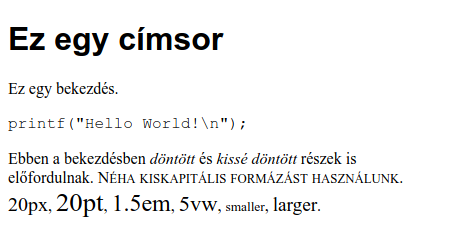
\includegraphics[scale=0.6]{karakter.png}
  \end{center}
\end{frame}

%61
\begin{frame}
  Karakterkészletek letölthetők a hálózatról: \texttt{@font-face}
  \begin{itemize}
    \item egyedi megjelenést kölcsönöz
    \item mindenki ugyanazt a készletet használja, garantáltan azonos megjelenés mindenhol (sok eszközön hiányosak a készletek, főleg a ritkán használt karakterek)
  \end{itemize}
  \vfill
  Megbízhatóan használható formátumok:
  \begin{itemize}
    \item \hiv{\href{https://en.wikipedia.org/wiki/TrueType}{TrueType Font (TTF)}}
    \item \hiv{\href{https://en.wikipedia.org/wiki/OpenType}{OpenType Font (OTF)}}
    \item \hiv{\href{https://en.wikipedia.org/wiki/Web_Open_Font_Format}{Web Open Font Format (WOFF)}}
  \end{itemize}
\end{frame}

%62
\begin{frame}
  A \texttt{@font-face} szabályban használható tulajdonságok:
  \begin{description}[m]
    \item[\texttt{font-family}] \hfill \\ Ezzel a névvel lehet majd hivatkozni a karakterkészletre később, kötelező.
    \item[\texttt{src}] \hfill \\ A fájl forrását adja meg \texttt{url()} CSS függvénnyel, kötelező.
    \item[\texttt{font-stretch}] \hfill \\ Ha a karakterkészletnek készültek különféle sűrűségű változatai, ezzel lehet kiválasztani, hogy valamelyiket milyennek tekintsen a böngésző (pl. \texttt{normal}, \texttt{condensed}, \texttt{expanded}). Ennek hiányában a böngészőnek kell előállíttatnia a speciális formákat a normálból kiindulva.
    \item[\texttt{font-style}] \hfill \\ Hasonlóan, dőlt változatokhoz (pl. \texttt{normal}, \texttt{italic}).
    \item[\texttt{font-weight}] \hfill \\ Hasonlóan, a ,,kövérséghez'' (pl. \texttt{normal}, \texttt{bold}).
  \end{description}
\end{frame}

%63
\begin{frame}
  \begin{columns}[c]
    \column{0.65\textwidth}
      \begin{exampleblock}{\textattachfile{webfont.html}{webfont.html}}
        \fontsize{7}{8} \selectfont
        \lstinputlisting[style=HTML,linerange={7-17},numbers=left,firstnumber=7]{webfont.html}
        \lstinputlisting[style=HTML,linerange={21-22},numbers=left,firstnumber=21]{webfont.html}
      \end{exampleblock}
    \column{0.3\textwidth}
      
\includegraphics[width=\textwidth]{webfont.png}
  \end{columns}
\end{frame}

%64
\begin{frame}
  \hiv{\href{https://developers.google.com/fonts}{Google Fonts}}
  \begin{itemize}
    \item Több száz ingyenes karakterkészlet
    \item Könnyű kereshetőség
    \item Egyszerű integráció a weboldalba
  \end{itemize}
\end{frame}

%65
\begin{frame}
  \begin{columns}[c]
    \column{0.65\textwidth}
      \begin{exampleblock}{\textattachfile{googleFonts.html}{googleFonts.html}}
        \scriptsize
        \lstinputlisting[style=HTML,linerange={6-12},numbers=left,firstnumber=6]{googleFonts.html}
        \lstinputlisting[style=HTML,linerange={15-15},numbers=left,firstnumber=15]{googleFonts.html}
      \end{exampleblock}
    \column{0.3\textwidth}
      
\includegraphics[width=\textwidth]{googleFonts.png}
  \end{columns}
\end{frame}

%66
\begin{frame}
  \begin{columns}[c]
    \column{0.5\textwidth}
      Készítse el Semmelweis Ignác oldalát a \hiv{\href{https://hu.wikipedia.org/wiki/Semmelweis_Ign\%C3\%A1c}{Wiki}} oldal szövegét felhasználva!
      \begin{itemize}
        \item Töltse le a \hiv{\href{https://befonts.com/ballerina-script-font.html}{Ballerina}} karakterkészletet!
        \item Használja ezt az első szintű címsorban szereplő név kiírására, 42 nyomdai pont méretben!
        \item A bekezdések szövegét írja \hiv{\href{https://fonts.google.com/}{Libre Baskerville}} karakterkészlettel, 12 nyodai pont mérettel!
        \item Készítsen stílusokat a félkövér és dőlt betűs részek megjelöléséhez!
      \end{itemize}
    \column{0.45\textwidth}
      \begin{exampleblock}{\textattachfile{semmelweis.html}{semmelweis.html}}
        \begin{center}
          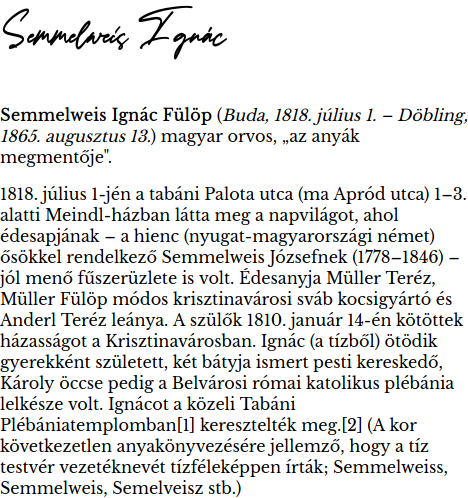
\includegraphics[width=0.7\textwidth]{semmelweis.png}
        \end{center}
      \end{exampleblock}
  \end{columns}
\end{frame}

% önálló feladat
